\chapter{Simulations}
\label{ch:simulations}

\section{Introduction}

In order to test algorithm ideas, one would either have to implement them as a prototype and run it on significant number of nodes, hoping that the results would scale in predictable way in relation to how node count changes. The other way is to create a simulator, which given input parameters - for example, the number of nodes, number of jobs and quality of nodes - would be able to estimate performance of the grid over time.

Simulator created for this thesis is able to test how would hypothetical computing grid behave, if jobs scheduling and trust management were implemented with methods and algorithms presented beforehand. The simulators are able to simulate dynamics of grid network during computation of one project. Network data, such as nodes' trust, times of completion and number of confirmations of jobs is collected.

Both simulators are implemented in C++, depending on standard C++ library. Parallel simulator uses OpenMPI. Gnuplot is used, along with gnuplot-iostream~\cite{gp-iostream} to plot the resulting data.

\section{Simulator design}

Simulator uses the notion of \emph{Nodes}, \emph{Jobs}, and \emph{Results}. Additionally, \emph{AssumedResult} is defined as the result that is hoped to be delivered by Node, but is not ready yet.

Node is described by:
\begin{itemize}
\item Performance - how quickly the node is able to generate new results.
\item Trust - current accumulated amount of trust from the confirming results.
\item Current job - job the node is currently computing.
\item Submitted results - collection of all submitted results.
\end{itemize}

Job is defined as:
\begin{itemize}
\item Difficulty - how difficult the task is to compute. Directly affects how long the node will spend on computing the task.
\item Results - collection of results already delivered.
\item Assumed results - collection of results that are hoped to be delivered.
\end{itemize}

Result is defined by \emph{hash}, which tells what kind of result it is. Hash value of 0 is considered as a correct result. Any other value makes the result to be considered incorrect, but the results with same hash value confirm one another. So enough incorrect but same results will be accepted as correct by the network, potentially disturbing its progress.

Each result is related to exactly one Node and exactly one Job. Result's \emph{correctness} is defined to be \emph{trust} of the \emph{node} at the time of submitting the result.

Relations between described classes are shown on figure~\ref{f:simclassdg}.

\begin{figure}
\centering
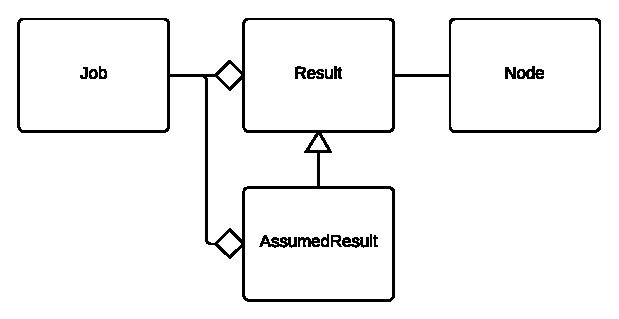
\includegraphics{diagrams/SimulatorClassDiagram.pdf}
\caption{Diagram of classes used in the simulator.}
\label{f:simclassdg}
\end{figure}

\section{Simulator loop}

Simulation is done by evaluating each node in a loop. Time is represented by abstract time unit called \emph{tick}. Every iteration of the loop is simulation of network in consecutive time units. In each iteration, every node is evaluated, by doing as follows:
\begin{itemize}
	\item If node is working on idling, continue to the next node.
	\item If not: \begin{itemize}
		\item If node has just finished job, hand out job, recompute job's correctness and participants' trust.
		\item Find a new job for the node. \begin{itemize}
			\item If job is found, calculate \emph{work time}.
			\item If no job is found, set to idle until next tick. 
		\end{itemize}
	\end{itemize}
\end{itemize}

The ticks are being simulated until all jobs are estimated to be complete. Job is complete when a set of results can be found which have the same \emph{hash} and sum of their \emph{correctness} exceeds $1$.

Upon each iteration, we can plot data such as nodes' trust or percent of completed jobs. Simulator uses gnuplot for this task.

\subsubsection{Work time}
\label{s:worktime}

The program simulates "work time" based on node's performance factor and job's difficulty factor. The work time is actually number of ticks that the node has to wait until it sends back the result and gets a new job. We assume that different nodes will get computing work done faster, and jobs may vary in difficulty, and therefore time to complete. All of this is simulated by the simulator software.

Work time is being calculated using following equation:
\begin{equation}
W(N, J) = 1 + 100 * \text{difficulty}(J) * (1 - \text{performance}(N))
\end{equation}
$W(N, J)$ being the work time (in ticks), $N$ being node for which it is calculated, and $J$ being the job.

Work time has a minimum value of 1, and is directly proportional to the difficulty factor of the job, and inversely proportional to node's performance factor. $100$ is used as a constant to scale work time from $1$ to $101$. In simulator, it needs to be a whole number. The fraction is dropped (results of the calculation is casted to an integer).

\section{Implementation}

We want to be able to simulate networks with hundreds of nodes and thousands of jobs. In order to achieve needed performance, appropriate data structures are used. This section will explain how certain performance critical aspects of simulator are implemented and the rationale behind it.

Set is used as a data structure to keep collection of objects. Ordered set can keep unique elements following a specific order. Operations on sets, such as searching for elements and inserting an element, are of logarithmic complexity.

\subsection{Nodes}

The node collection is an ordered set, where the order is determined by \emph{next working tick}. \emph{Next working tick} is the tick when the node state should change. When a node gets job at tick $10$ and the job is calculated to take $5$ ticks, \emph{next working tick} is $15$. At tick $15$ job will be finished, nodes' trust recalculated and node will get new job. There is no need to check on the node in ticks $11$ to $14$.

\begin{figure}
\centering
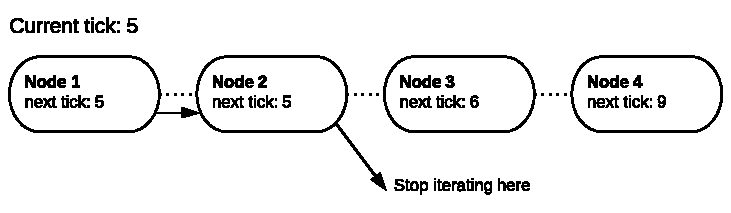
\includegraphics{diagrams/SimulatorNodes.pdf}
\caption{Iterating through simulator nodes. Simulator breaks out of the loop early, skipping nodes that should not be processed in current iteration.}
\label{f:simnodes}
\end{figure}

Because iteration happens on ordered set of nodes, we can stop iterating as soon as we reach node that \emph{next working tick} is higher than current tick. Example of this behavior is shown in figure~\ref{f:simnodes}. The only thing to keep in mind is to reinsert node (to update its position in set and keep set's consistency) when node state is changed and therefore \emph{next working tick} changes.

\subsection{Jobs}

Jobs are kept in ordered set with the order determined by jobs current best correctness, but in reverse. Jobs with highest correctness are first. Because we search a job for nodes very often, it can become performance bottleneck. 

Jobs are selected in a way that node's contribution will get job closer to completion, which is determined by sum of trust of confirmed results of $1$, but also trying not to waste node's computing power. Waste is considered when sum of correctness exceeds $1$ by significant amount. For example, when job's best correctness is $0.8$, there is no reason to give this job again for a node with trust of $0.5$. Node with $0.2$ trust will suffice.

Ordered set of jobs allows us to use bisection to find best matching job. It may happen that the job cannot be given to this particular node, because it already has sent result for it. If so, we start iterating from that node until we find one that we can give to the node.

Failure in finding a job for a node is not an error. The simulator will try again in next tick - state of the network will be changed, and the search may succeed then.

\section{Simulation results}

This section describes experiments performed using the simulator and reason about inner working of the algorithms trying to understand observed behavior. 

\subsection{Dishonest nodes}

The first experiment was to measure performance of the network with dishonest nodes. We call dishonest node a node that is randomly sending back incorrect results with probability $P$. The nodes are not colluding with one other, each dishonest node is replying with its own, random, incorrect result, in hopes that it would be accepted by network as a correct one.

We measured average number of results a job needed to have before it was done. The test was performed with different ratio of dishonesty. Figure~\ref{f:confirmations1} shows results of first test. The simulated network had $100$ nodes and $5000$ jobs. Different dishonesty ratios were applied, to all of the nodes, varying from $P = 0.0$ to $P = 0.5$. Dishonesty ratio of $0.0$ means that the node always sends correct results, ratio of $0.5$ means that there is only $50\%$ chance of the node sending correct results. With dishonesty ratio higher than $0.5$, the network was behaving in very erratic way, and very low amount of jobs was being completed.

Average number of confirmations is $\approx 2.15$ when dishonesty ratio is $0$. Reason for this number being higher than $2$ is that the average from the entire project is taken, and when the project starts and trust is not yet established, the number of confirmations is higher.

\begin{figure}
\centering
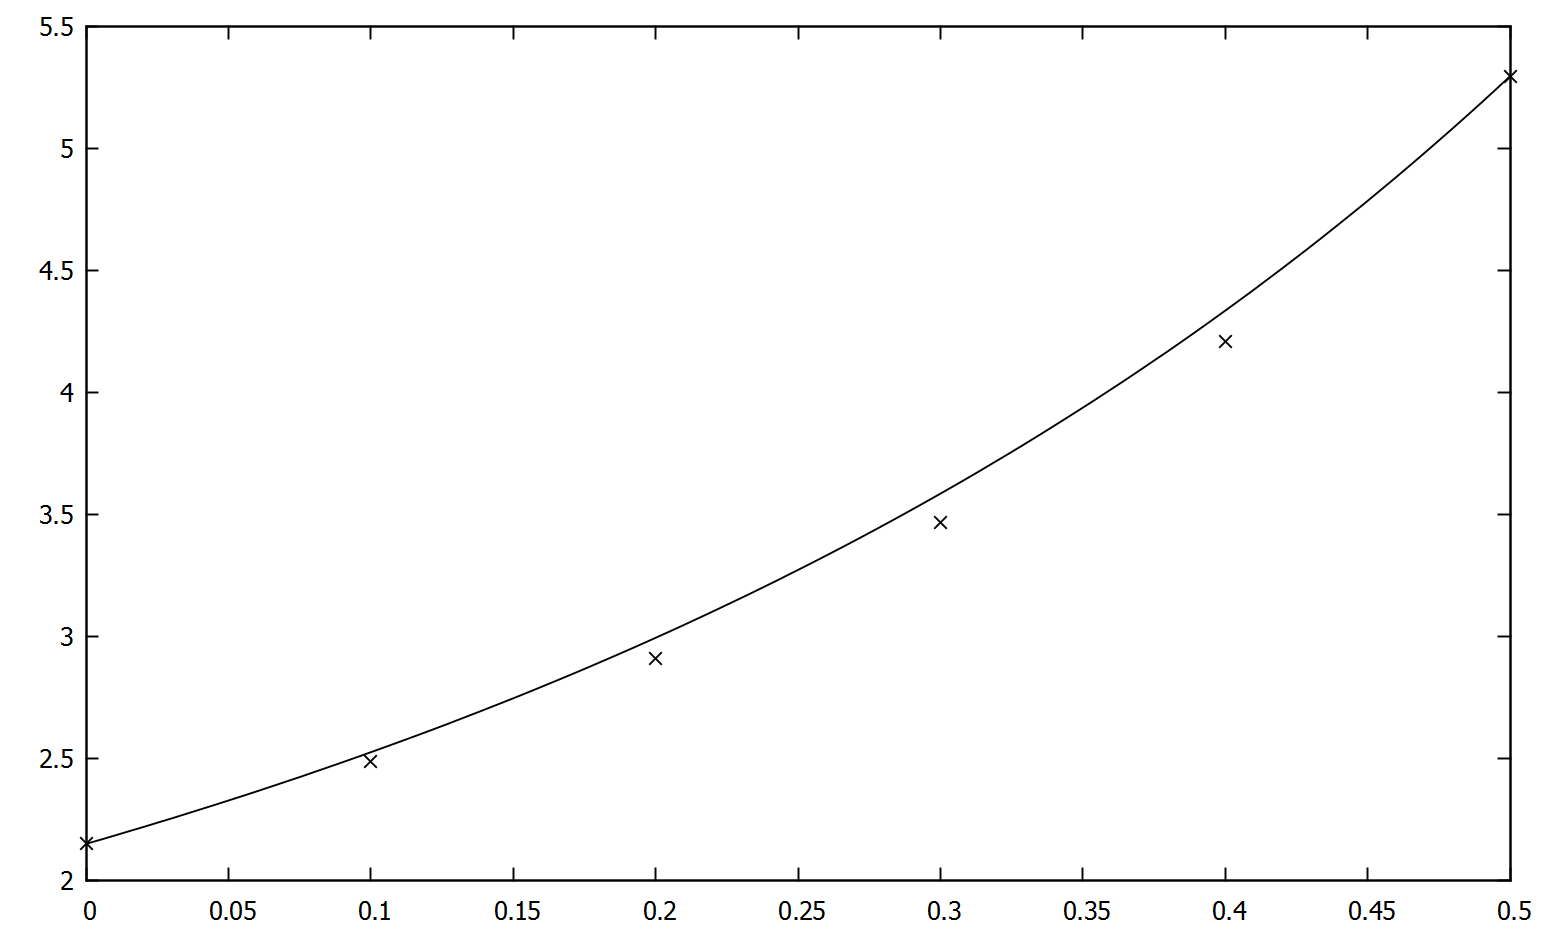
\includegraphics[width=\textwidth]{diagrams/confirmations.png}
\caption{First experiment with dishonest nodes: average number of confirmations (on Y axis) per dishonesty ratio of network (on X axis).}
\label{f:confirmations1}
\end{figure}

Described test simulates environment where the whole network is for some reason inconsistent with results. Another test was performed, that should resemble real life scenario more. In the second test, a part of network has been set to have dishonesty ratio of $0.5$. The rest of it was always honest (ratio of $0.0$). The simulated network also had $100$ nodes and $5000$ jobs. Simulations were performed using different number of dishonest nodes (all with dishonesty ratio of $0.5$). Figure~\ref{f:confirmations2} shows results of the simulation. Network behaves reasonably well even with high number of dishonest nodes. Even when $60\%$ of the nodes send incorrect results, trust model managed to isolate them in a way that network operations were not affected all that much - jobs still needed less than 3 results on average to be confirmed to be correct. For the highest value we tested, $80\%$ of dishonest nodes, the network needed $\approx 4.2$ confirmations on average to mark the job as done.

\begin{figure}
\centering
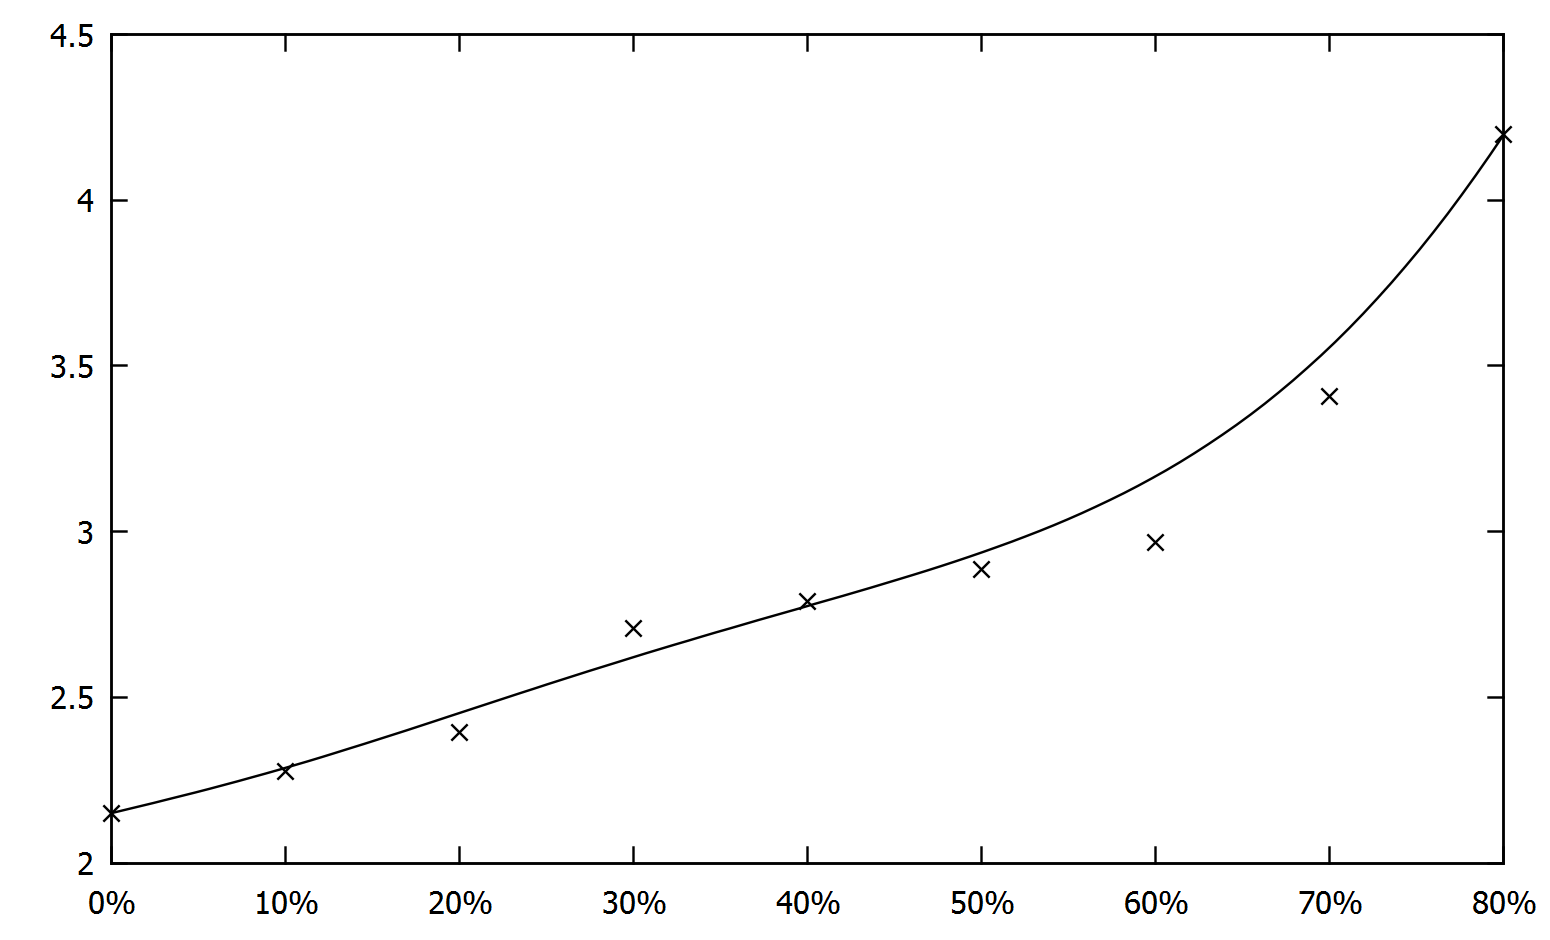
\includegraphics[width=\textwidth]{diagrams/confirmations2.png}
\caption{Second experiment with dishonest nodes: average number of confirmations (on Y axis) per ratio of dishonest nodes (on X axis).}
\label{f:confirmations2}
\end{figure}

Important fact is that all the dishonest nodes were not colluding. When they were to submit an incorrect result, a random one was chosen. For every experiment, no incorrect result was accepted as a correct one. A real life attack on a network would probably consist of many nodes colluding with each other and sending same (but incorrect) results for one problem, which would force the network to accept it as right, if the number of nodes was high enough. Analyzing and defending from such attacks is out of scope of this thesis.

\FloatBarrier

\subsection{Joining and leaving the network}

The next experiment shows change of trust of nodes over time. All simulations have been performed on a network that has $10,000$ jobs and $500$ nodes. All nodes were set to be always honest. Their performance was randomly assigned, as well as job difficulty, which was also random. All nodes have base, constant, trust of $0.1$. Adding a constant trust factor helps the nodes to reach their peak trust faster.

Figure~\ref{f:trust1} shows trust over time of $3$ selected nodes. \emph{Node $2$} is visibly more performant than the other two. We can observe nodes' trust dropping when they are busy computing work, and going back up when they send back the result. The changes are more rapid at the beginning, when nodes still have not performed too much work and slightest change of trust has big effect globally. 

\begin{figure}
\centering
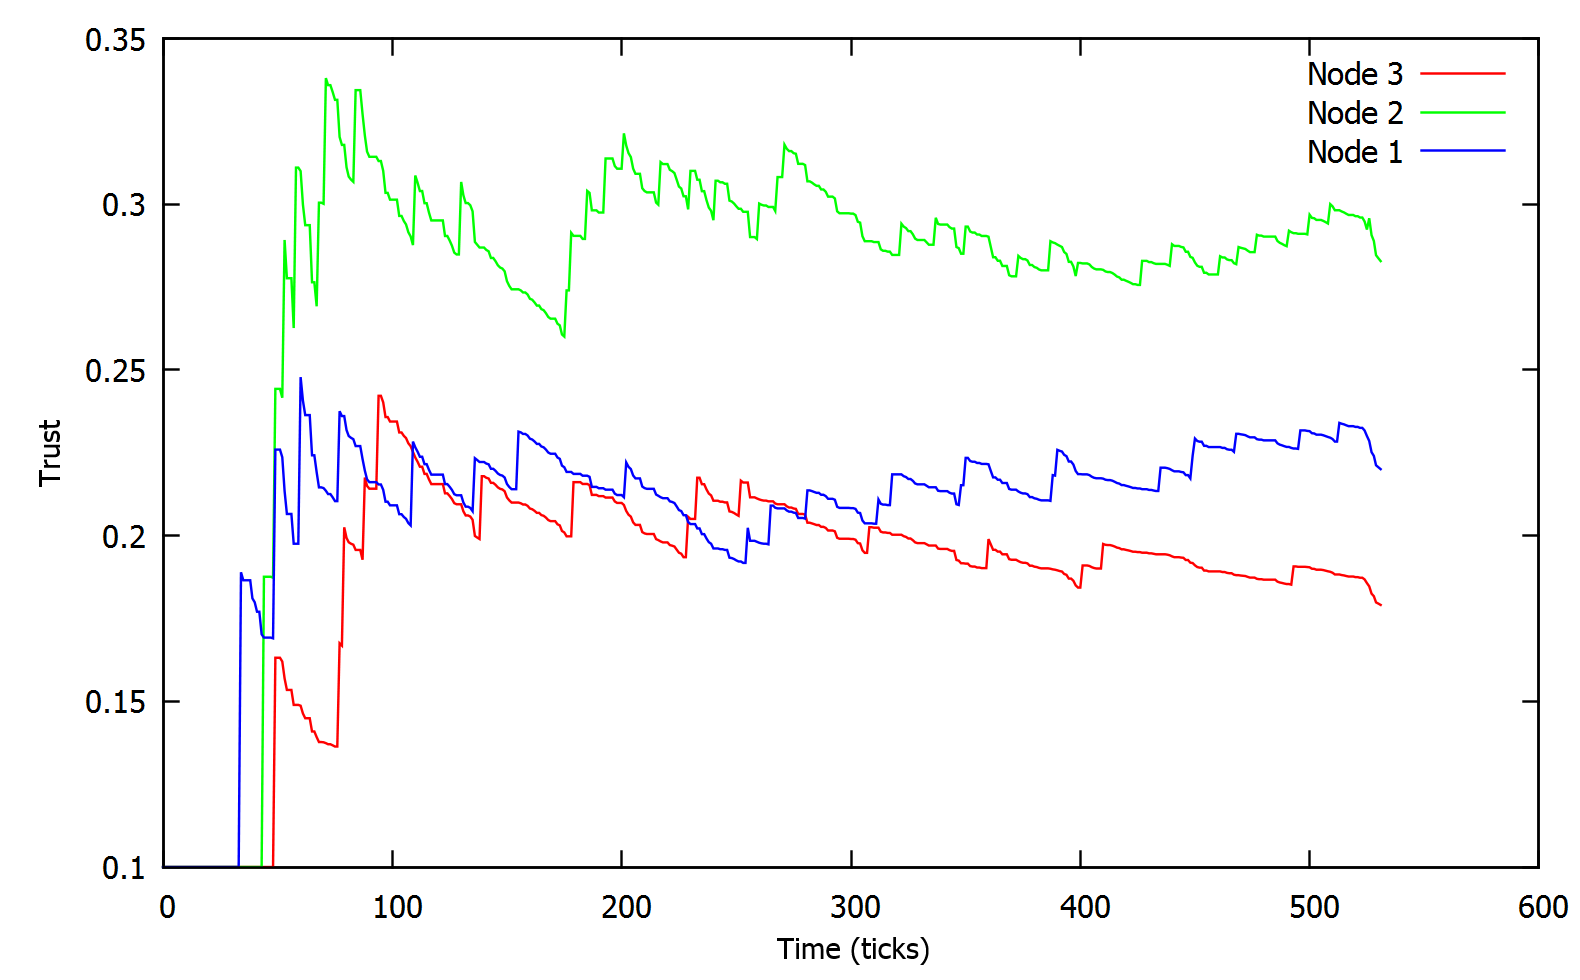
\includegraphics[width=\textwidth]{diagrams/trust1.png}
\caption{Trust of 3 selected nodes during network simulation. Trust is on the Y axis, time (in ticks) on the X axis.}
\label{f:trust1}
\end{figure}

Then, we simulated a network in which one of the nodes joins in the middle of computing project. We can observe its trust quickly growing and reaching its peak, which depends on node's performance factor. Figure~\ref{f:trust_join} shows results of the simulation. \emph{Node 1} is the node joining the project in tick $150$. 

\begin{figure}
\centering
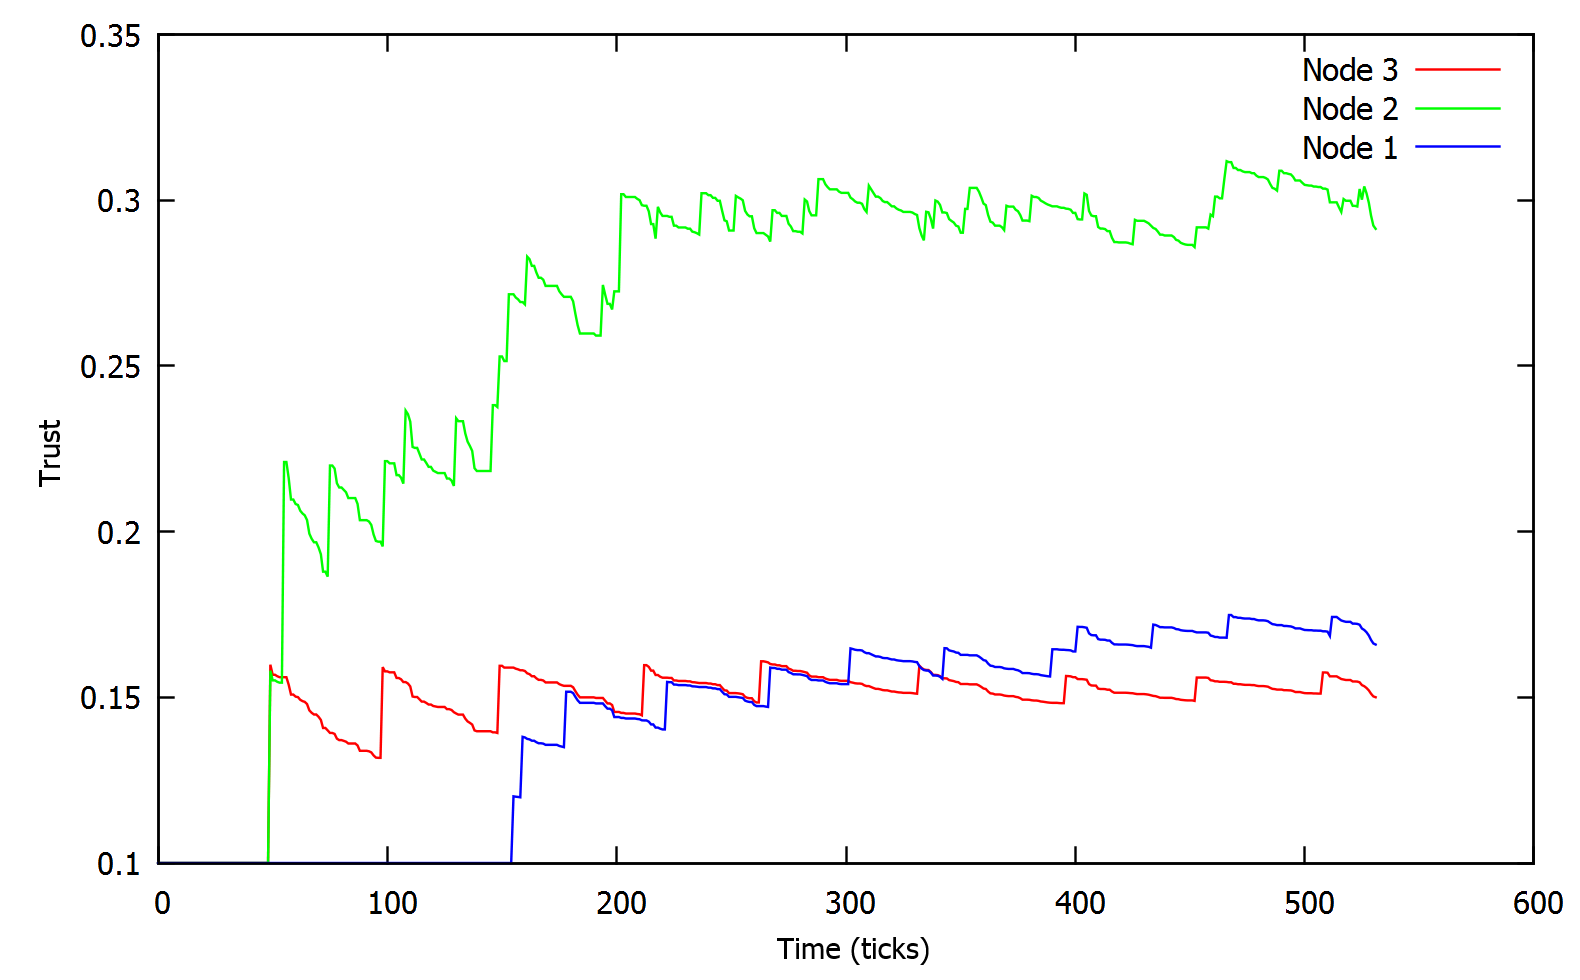
\includegraphics[width=\textwidth]{diagrams/trust_join.png}
\caption{Experiment with node joining the network. Trust is on the Y axis, time (in ticks) on the X axis.}
\label{f:trust_join}
\end{figure}

One simulation was conducted with node leaving the network in the middle of project. Figure~\ref{f:trust_leave} shows the plot of nodes' trust during the simulation. \emph{Node 1} has stopped computing work in tick $250$ and its trust has been getting lower since. Because the project ended around tick $500$, we do not get to observe \emph{Node 1} trust falling all the way to the bottom, but that is what would have happened.

\begin{figure}
\centering
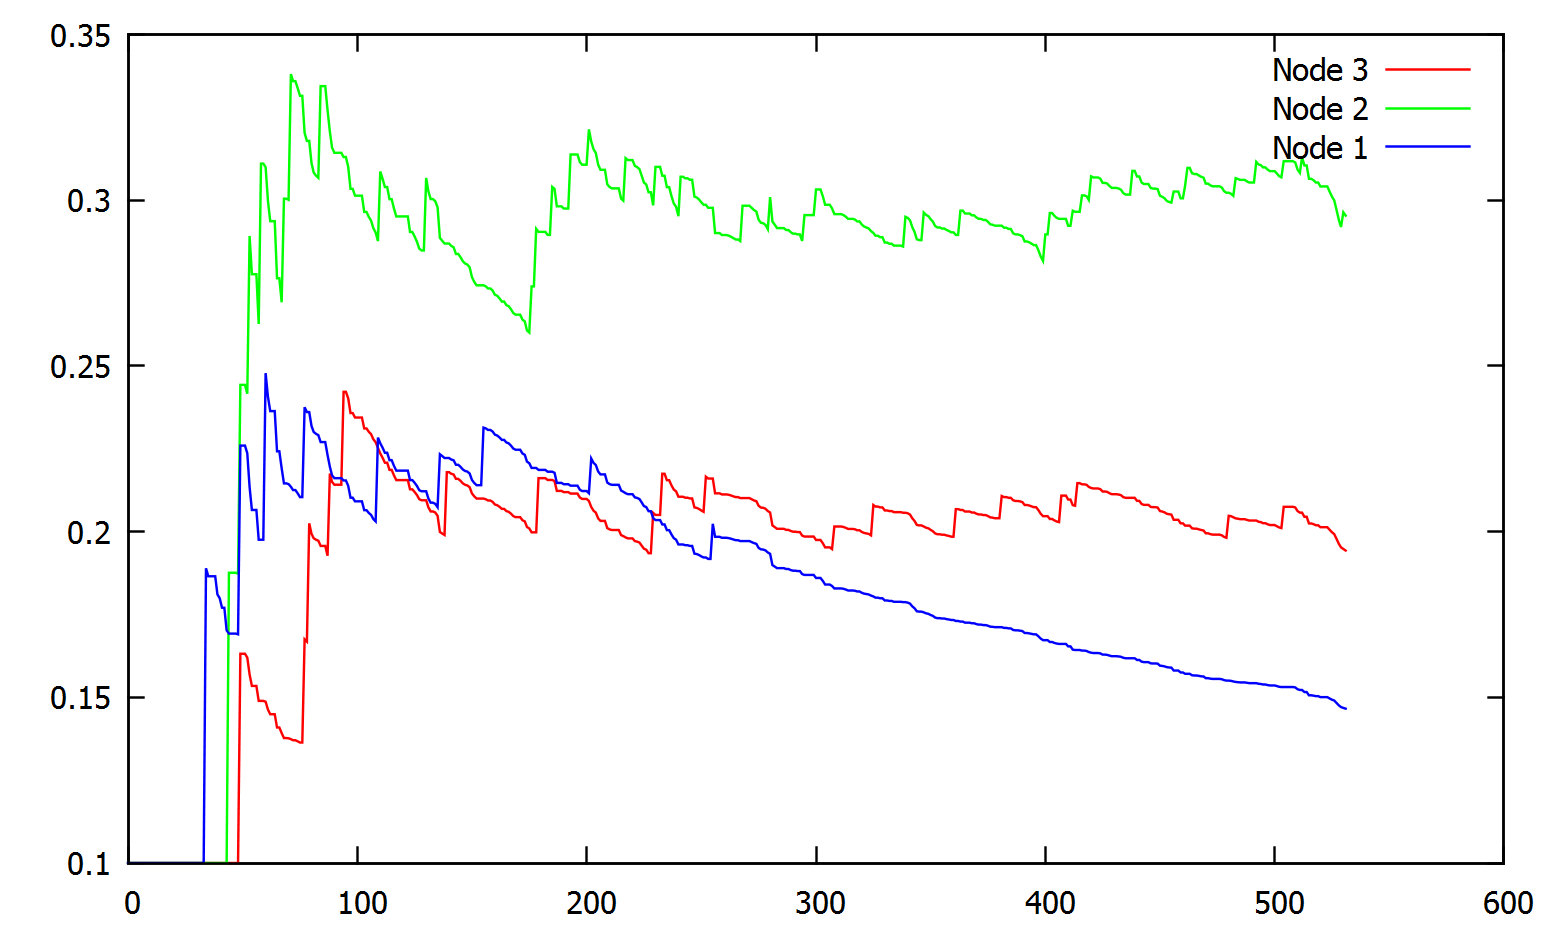
\includegraphics[width=\textwidth]{diagrams/trust_leave.png}
\caption{Experiment with node leaving the network. Trust is on the Y axis, time (in ticks) on the X axis.}
\label{f:trust_leave}
\end{figure}

\FloatBarrier

\subsection{Inconvenient cases}

Next, we tested inconvenient cases for the simulation. First one is where there are very few jobs in comparison to the number of nodes. For the simulation, we used a network in which there was only $500$, and $500$ nodes. The results, plotted on figure~\ref{f:less_jobs}, shows that the network can handle such situation as well. The nodes had problem at the beginning to receive jobs (because the competition was high), but it managed to stabilize and the plots look as expected, although in smaller scale - such project was completed very quickly. The average number of sent results per job was $\approx 3.74$. The reason is that the nodes did not get a chance to reach their peak trust.

\begin{figure}
\centering
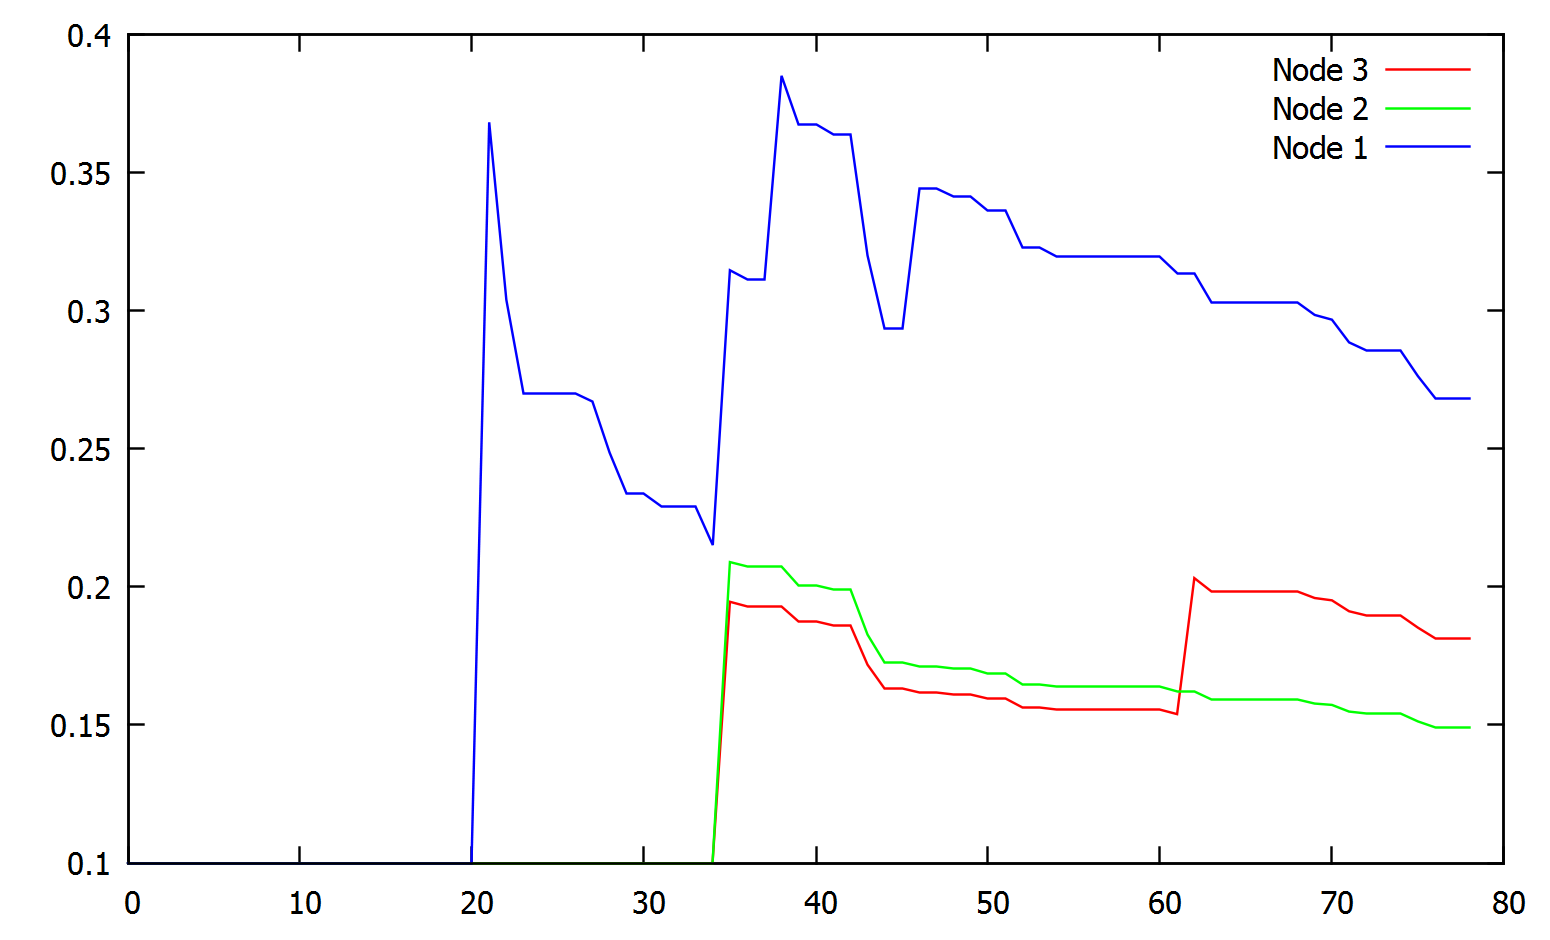
\includegraphics[width=\textwidth]{diagrams/trust_less_jobs.png}
\caption{Experiment where the network had same number of jobs and nodes. Trust is on the Y axis, time (in ticks) on the X axis.}
\label{f:less_jobs}
\end{figure}

Second case is where the network has many jobs but less nodes. The simulation was run with $5000$ jobs but only $50$ nodes. Resulting plot is on figure~\ref{f:more_jobs}. The stabilization phase is longer at first, but then the network behaves normally. It reaches $\approx 2.08$ results per completed job, which is the lowest number achieved in the simulations. This means, that generally it is healthier for the network to have higher number of jobs per node. The network took long to finish the project, but that was expected with amount of nodes this little for project that big.

\begin{figure}
\centering
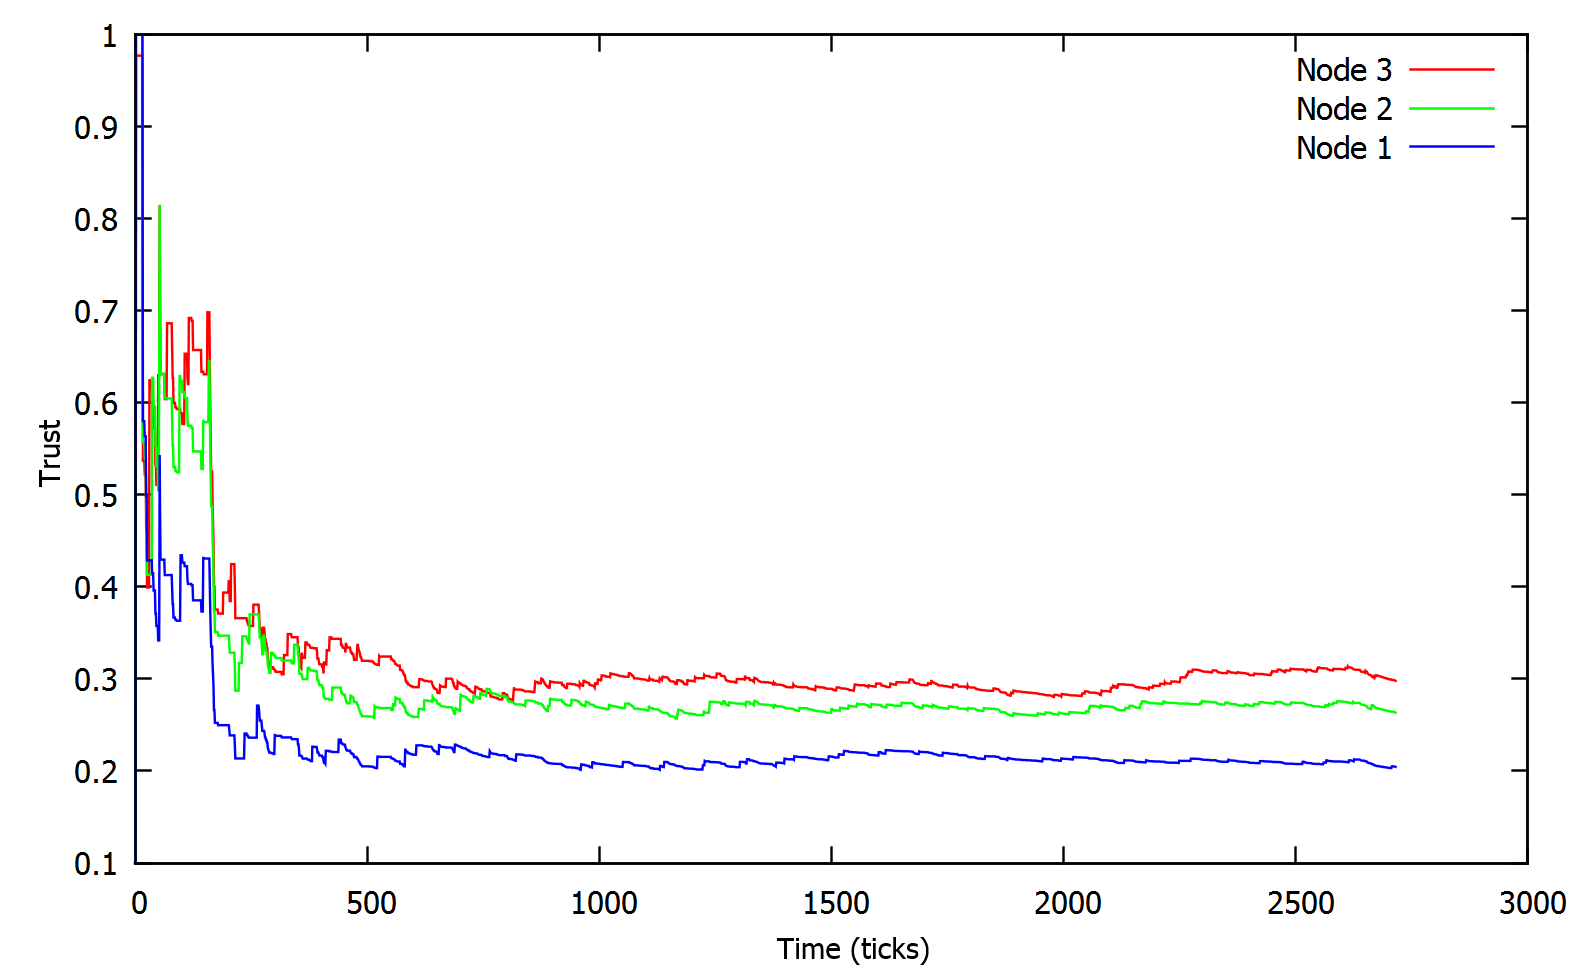
\includegraphics[width=\textwidth]{diagrams/trust_less_nodes.png}
\caption{Experiment with low number of nodes. Trust is on the Y axis, time (in ticks) on the X axis.}
\label{f:more_jobs}
\end{figure}

\FloatBarrier

\subsection{Case of homogeneous network}

In all previous cases, the nodes performance was evenly distributed. This case shows a network where all nodes have the same performance. Results are plotted on figure~\ref{f:evenly}. The project had $10,000$ nodes and $1000$ jobs. We can observe that competition was very high and all nodes had very high trust, approaching $1$.

The network still worked and managed to complete the project. The average number of results per job was $\approx 2.19$. Although this is not a normal case for volunteer networks, it is not uncommon with computing grids, where all of the hardware is similar or even the same. This experiment shows that the trust model can be used with clusters of homogeneous hardware.

\begin{figure}
\centering
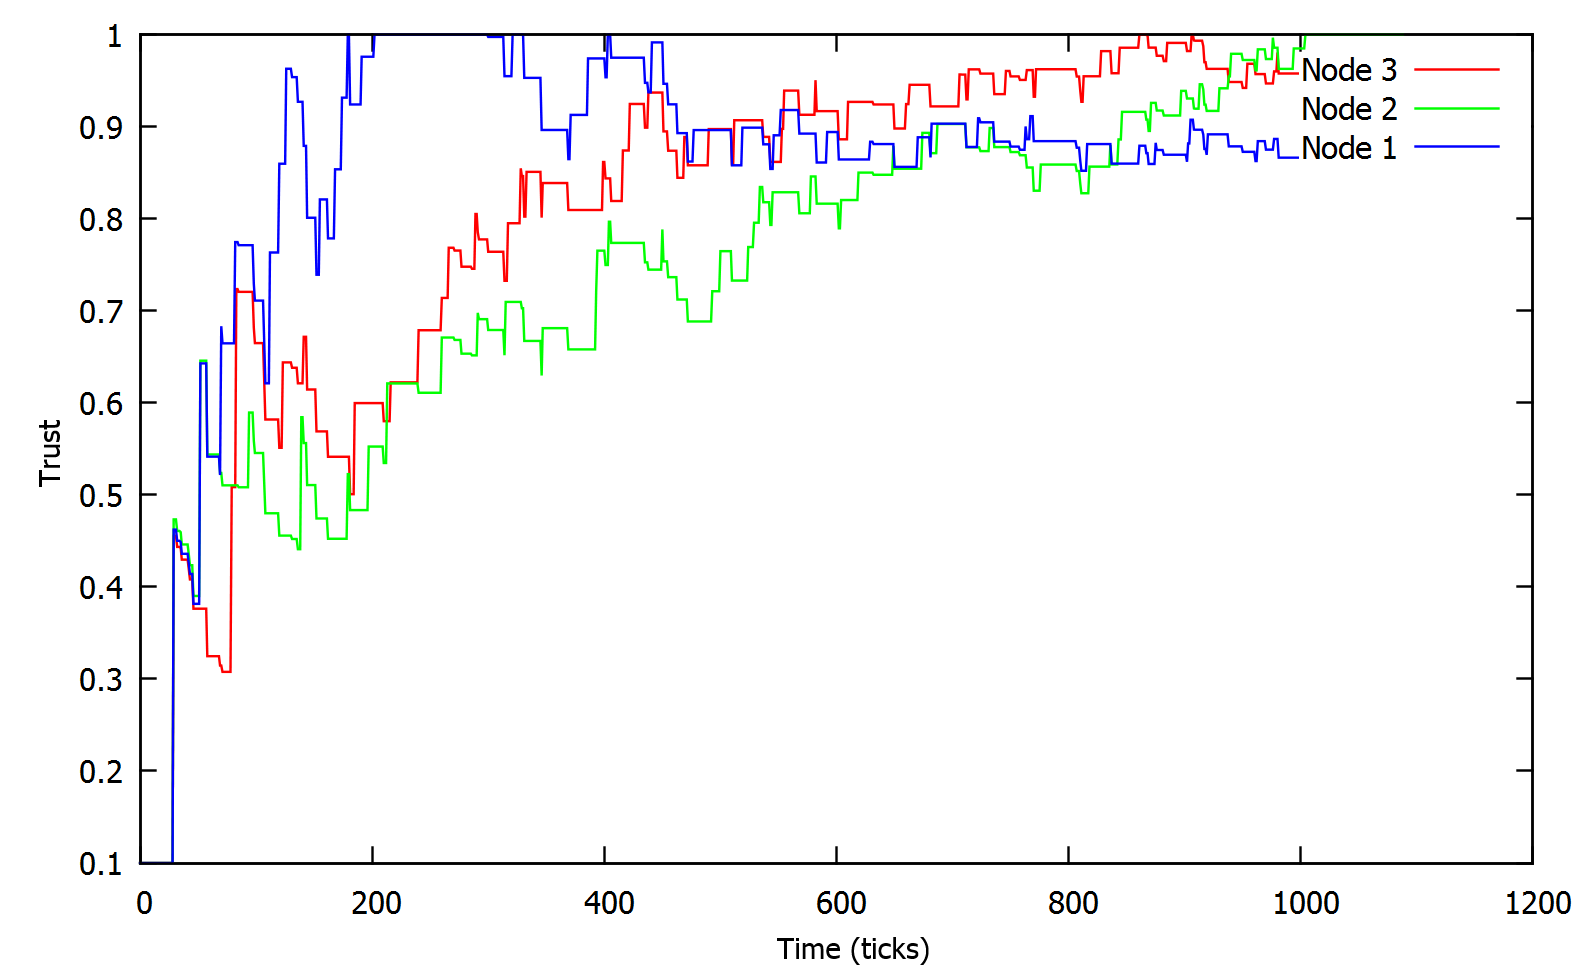
\includegraphics[width=\textwidth]{diagrams/trust_static.png}
\caption{Experiment with network of homogeneous performance. Trust is on the Y axis, time (in ticks) on the X axis.}
\label{f:evenly}
\end{figure}